\subsection{Vehicle Volume Counting}
\label{subsection:count_measure}

This component of the algorithm takes as input the tracked object data from the object tracking component and returns updated traffic data for vehicle volumes. 

\subsubsection{Counting}

Depending on the direction of travel relative to the image, that is, up or down vs side to side, a line is specified on the image which when passed by a tracked object triggers a vehicle to be counted. The direction of travel of the object is determined by averaging the vehicle's position history. Figure \ref{fig:count_lines} shows an example of a count line. Algorithm \ref{algorithm:count} details the process of determining if a vehicle has crossed a count line.

\begin{algorithm}
	\SetAlgoLined
	\KwInput{List of tracked objects, \emph{tobjs}} 
	\KwOutput{Updated vehicle volume statistics}
	\For{\emph{obj} in \emph{tobjs}}{
		get average direction of \emph{obj}\;
		get start position of \emph{obj}\;
		\If{obj most recent position opposite side of line start position}{
			increment volume count for \emph{obj} travel direction\;
		}
	}
	\caption{Centroid re-assignment algorithm. \cite{adrian_rosebrock_vehicle_tracking}}
	\label{algorithm:count}
  \end{algorithm}

\begin{figure}[H]
	\centering
	\begin{subfigure}[b]{0.42\textwidth}
            \centering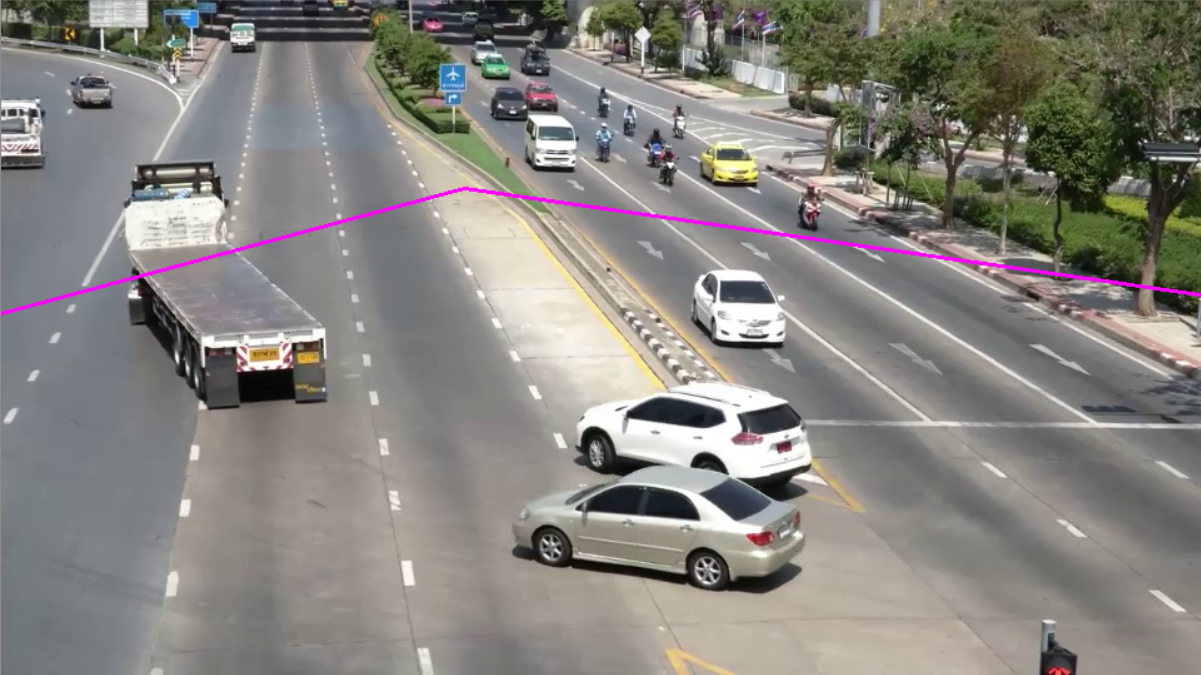
\includegraphics[width = \textwidth]{design/detection/counting/updowntraffic.png}|
            \captionsetup{format = hang}  
      		\caption{Count lines for traffic travelling up and down.}
    	\end{subfigure}
    	\begin{subfigure}[b]{0.42\textwidth}
      		\centering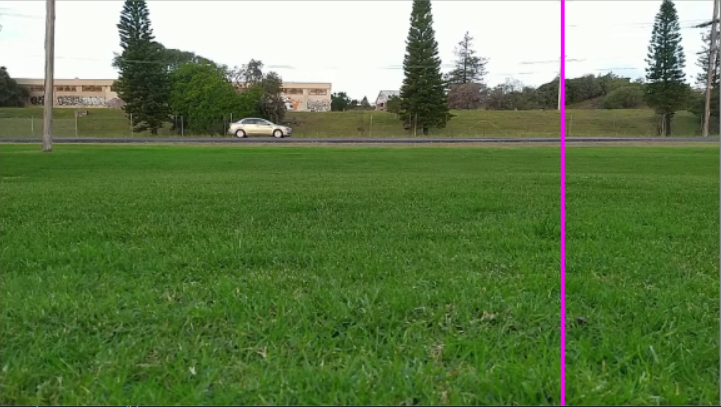
\includegraphics[width = \textwidth]{design/detection/counting/leftrighttraffic.png}
            \captionsetup{format = hang}    
            \caption{Count line for traffic travelling left and right.}
        \end{subfigure}
        \captionsetup{format = hang}
    	\caption{Count line visualization for both traffic direction orientations.}
    	\label{fig:count_lines}
\end{figure}

% \subsubsection{Speed Estimation}

% Time stamps associated with a vehicle's location history allow the speed of that vehicle to be estimated. Similar to when counting, two lines are placed on the image and when a vehicle travel between them it's speed over that region is measure. This is achieved by converting the distance travelled in pixels into meters. Figure \ref{fig:speed} shows an example highlighted region in which a vehicle's speed is measured.  For a camera perspective looking in the direction of travel as in Figure \ref{fig:original_frame} and not perpendicular to it, the accuracy will be reduced. This is because object scale changes with distance from a node. In a situation where vehicles are travelling perpendicular to the camera's perspective their size remains constant and hence perceived pixels per time unit doesn't change as they move. This type of speed measuring is referred to as \emph{Visual Average Speed Computer and Recorder} (VASCAR) as it relies on visual inputs to determine a vehicles speed, it is less accurate than other methods like radar but is sufficient for the purpose of measuring approximate traffic speed to gauge traffic flow in conjunction with vehicle volumes.

% \begin{figure}[H]
% 	\centering
% 	\centering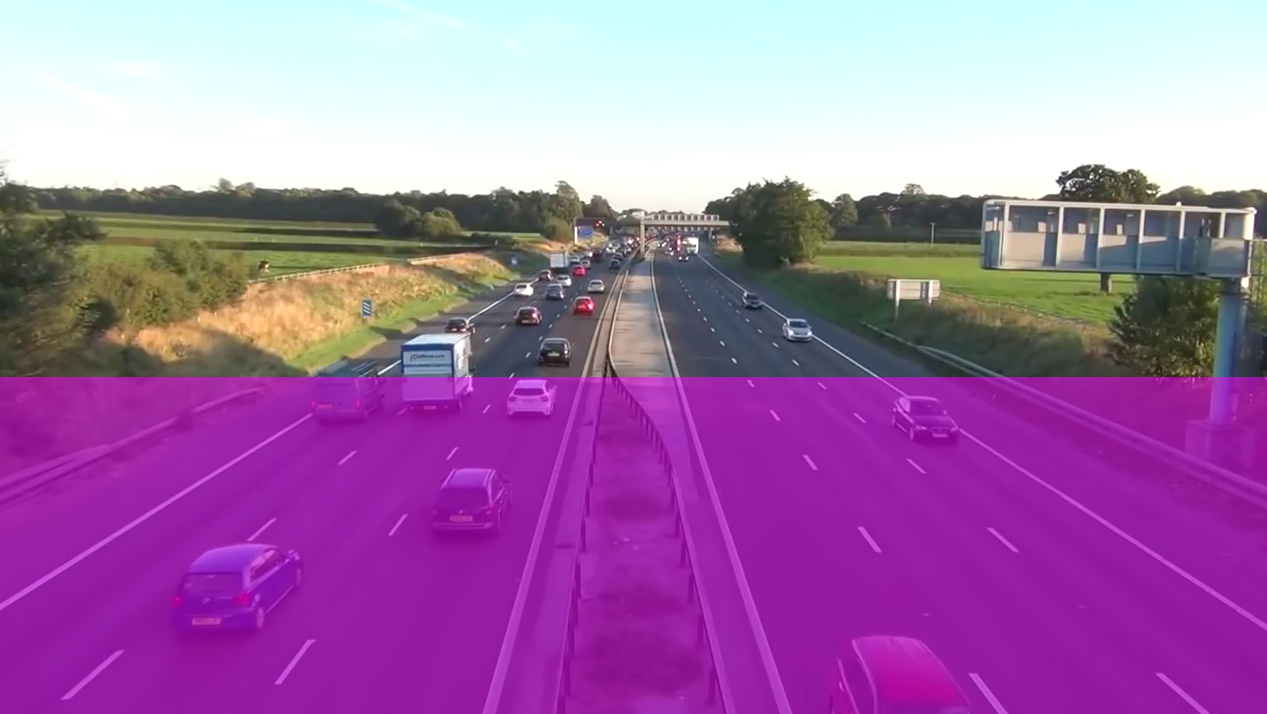
\includegraphics[width = 0.8\textwidth]{design/detection/counting/original_speed}
% 	\caption{Visualization of speed measurement region.}
% 	\label{fig:speed}
% \end{figure} 

\subsubsection{Calibration}

The calibration of volume counting depends mostly on the position of the count line. Because not all camera perspectives are optimal the count line should be placed where the most correct readings are generated. To this end the system is capable of placing two count lines where it is intended that one line be used for each direction of traffic if there's more than one. 

The process of validating a vehicle crossing also considers how many frames has a vehicle has been tracked for, \emph{history\_count}, how many frames was a vehicle tracked on the side of the line opposite to its destination, \emph{otherside\_centroids}.  It's more likely that an object is legitimate if it has been tracked for a substantial amount of time because if it's noise or some anomalous entity it will usually be cleaned up by the background subtractor or morphology eventually. The intention \emph{otherside\_centroids} is to false positives generated by noise close to a count line that creates centroids that jump from side to side.
  